%\documentclass[journal]{IEEEtran}
\documentclass[conference]{IEEEtran}
%\documentclass[twocolumn]{article}

% Begin IEEE recommended very useful LaTeX packages:
\usepackage{cite}
\usepackage{graphicx}
\usepackage{epsfig}
\usepackage{psfrag}
\usepackage{subfigure}
\usepackage{url}  
\usepackage{array}
\usepackage{amsmath}
\interdisplaylinepenalty=2500
% End IEEE recommended very useful LaTeX packages:

\newcommand{\var}[1]{{\footnotesize #1}}

% correct bad hyphenation here
\hyphenation{op-tical net-works semi-conduc-tor IEEEtran}

\begin{document}

\newlength{\pin}
\setlength{\pin}{0.2in}
\newcommand{\email}[1]{\textless #1\textgreater}
%\newcommand{\helm}{IvP Helm}
%\newcommand{\phelm}{pHelmIvP}
%\newcommand{\ibuff}{info\_buffer}
\newcounter{listing}
\newcounter{alisting}

\newenvironment{hangpar}[1]{\list{}{
    \setlength{\listparindent}{1.5em}       \setlength{\itemindent}{0pt}
    \setlength{\itemsep}{0pt}               \setlength{\parindent}{0pt}
    \setlength{\rightmargin}{0pt}           \setlength{\leftmargin}{#1}
               \parsep                                 \medskipamount}%
    \item\hspace{-\leftmargin}\noindent\ignorespaces}
    {\endlist}


\title{A Guide to Artifact Searching using MOOSIvP}


\author{Andrew Shafer, Michael Benjamin \\
Dept of Electrical Engineering/Computer Science, MIT \\
Cambridge MA 02139 \\
\email{ajshafer@mit.edu}, \email{mikerb@mit.edu} \\ \\
{\Large{\today}}}
\maketitle



\begin{abstract}
This is the abstract.
\end{abstract}

\section{Introduction}
\label{intro}

This document describes the use and development of the artifact search system developed as a Master's of Engineering thesis by Andrew Shafer at MIT.  This document assumes that the reader has a familiarity with MOOS and IvP and understands how to use those tools (see \cite{new03}, \cite{ben02a}, \cite{ben03}, and \cite{ben04b}).

First, a bit of terminology.  In this document, an "artifact" is an object of interest.  An artifact can be any detectable, identifiable object.  In a naval application this would commonly be some type of mine.  In naval terminology, "mine-hunting" (or mine-sweeping) usually refers to the process of detecting mines and deactivating or destroying them.  "Mine-searching," on the other hand, refers to simply mapping out the locations of detected mines for later deactivation/destruction.  Therefore, this project is more properly an artifact searching system, rather than a mine-hunting system.

A "search area" is the geographic region that the user desires to search (see Figure~\ref{searcharea}).  This area is broken up into uniform, discrete cells that together constitute the "search grid" (see Figure~\ref{searchgrid}).

\begin{figure}[ht]
\label{searcharea}
\begin{minipage}[c]{0.5\textwidth}
  \centering 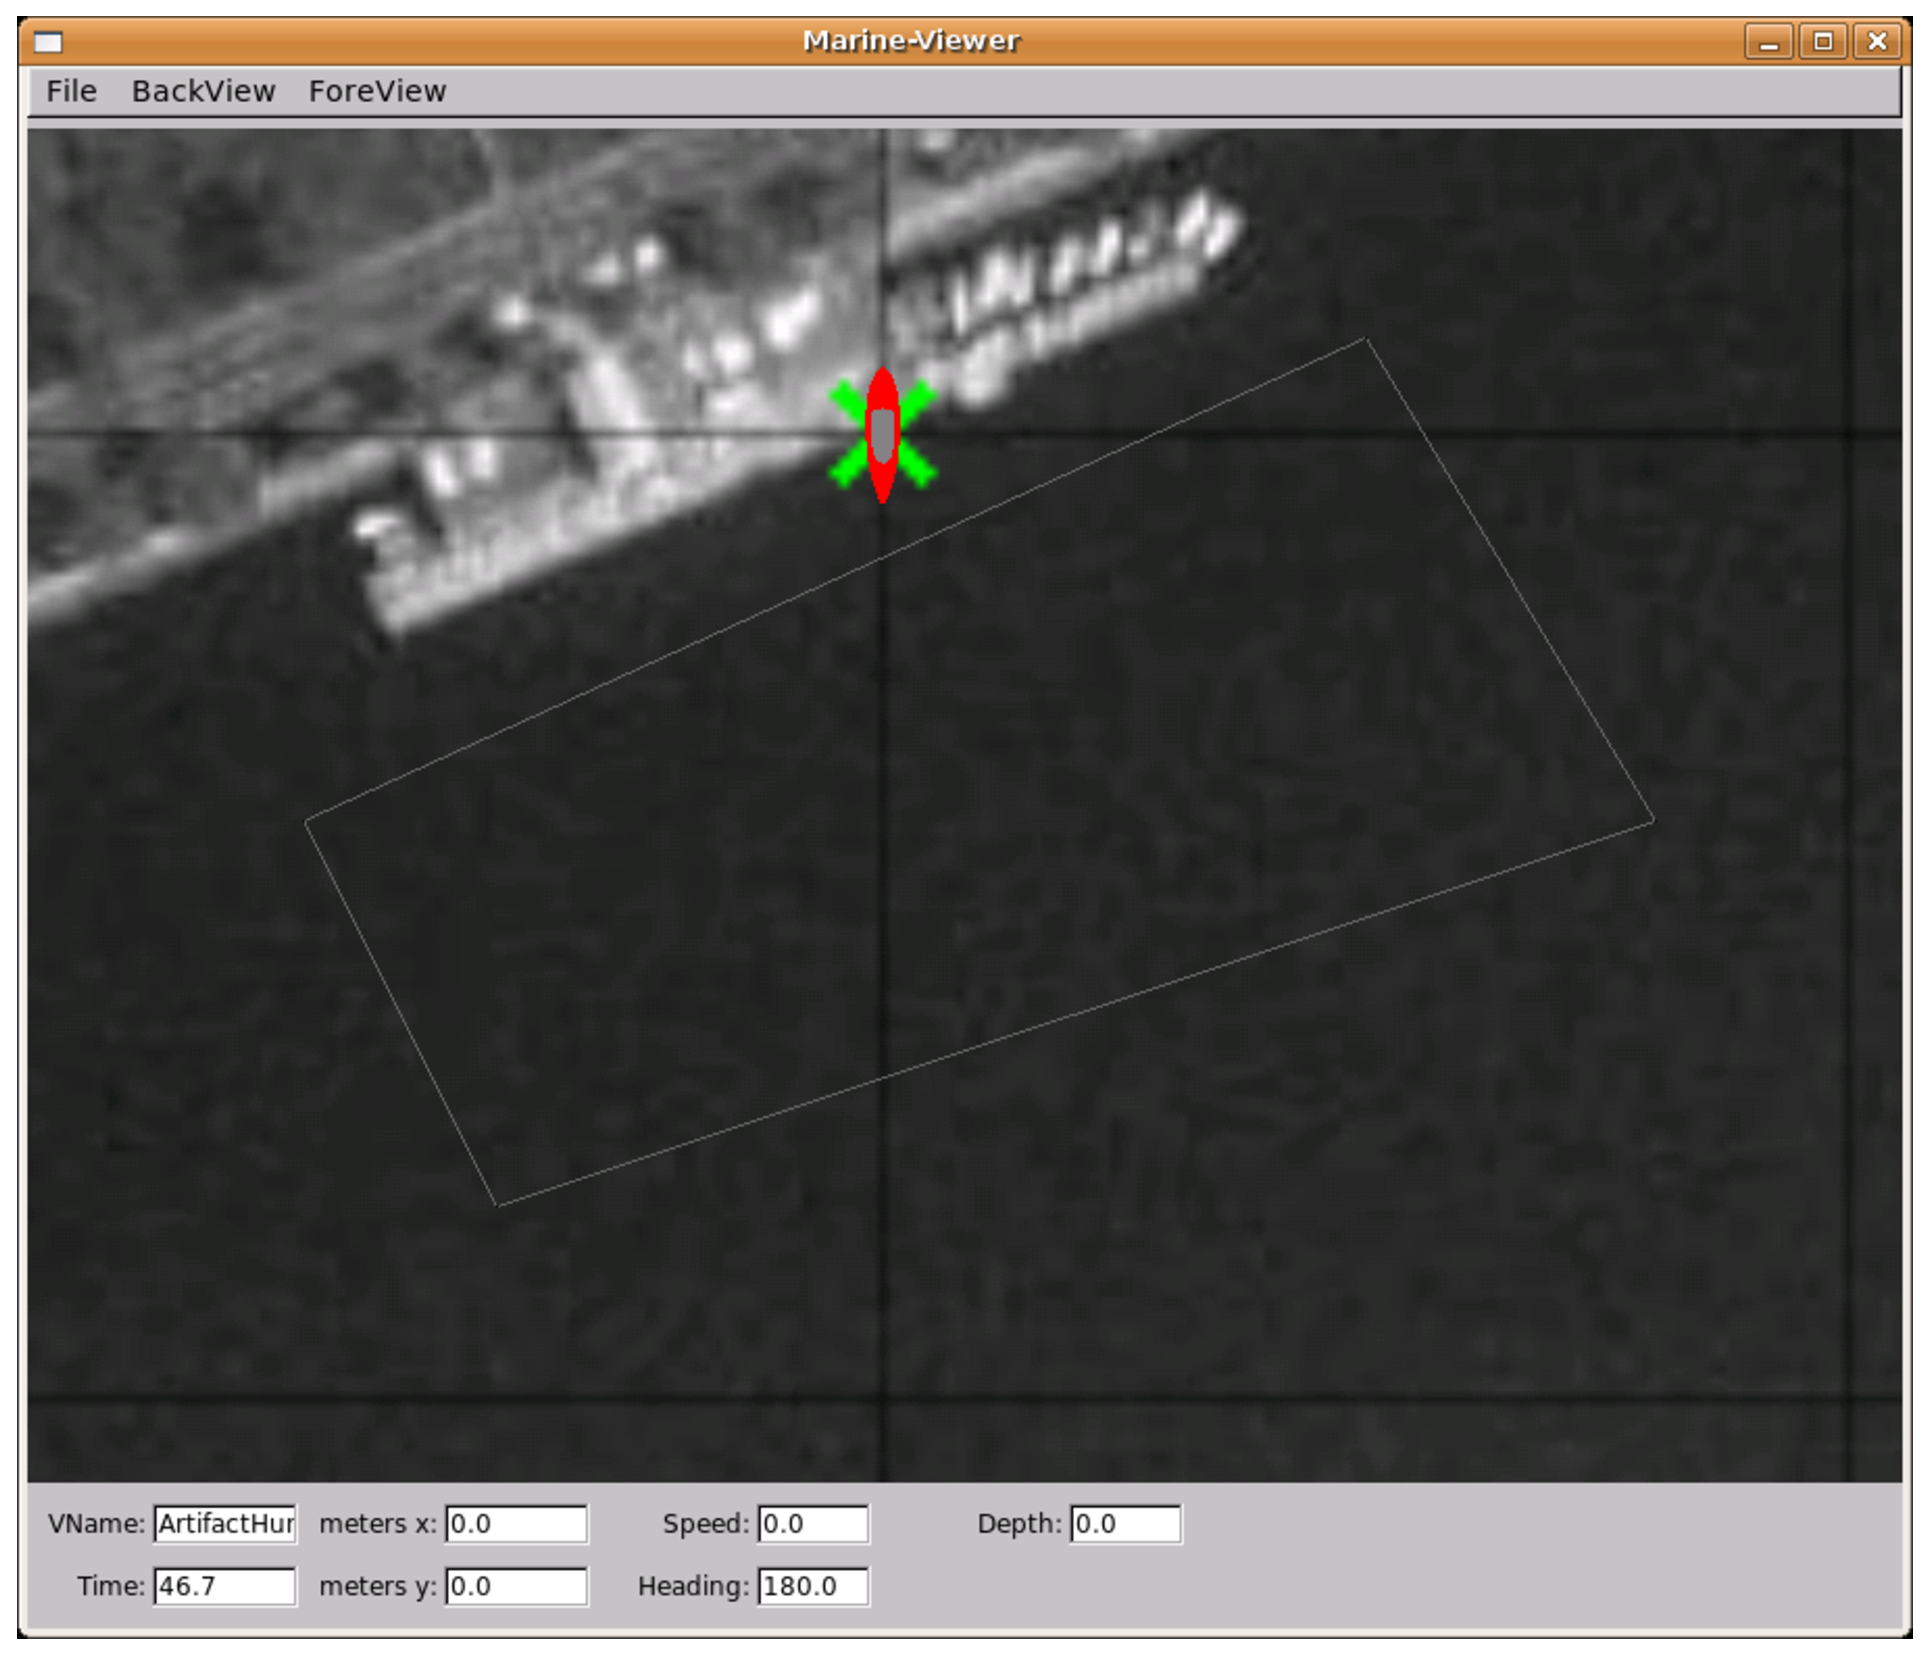
\includegraphics[width=2.5in]{figures/searcharea}
\end{minipage}
\caption{A geographic area (a convex polygon) defined as a search grid.}
\end{figure}

\begin{figure}[ht]
\label{searchgrid}
\begin{minipage}[c]{0.5\textwidth}
  \centering 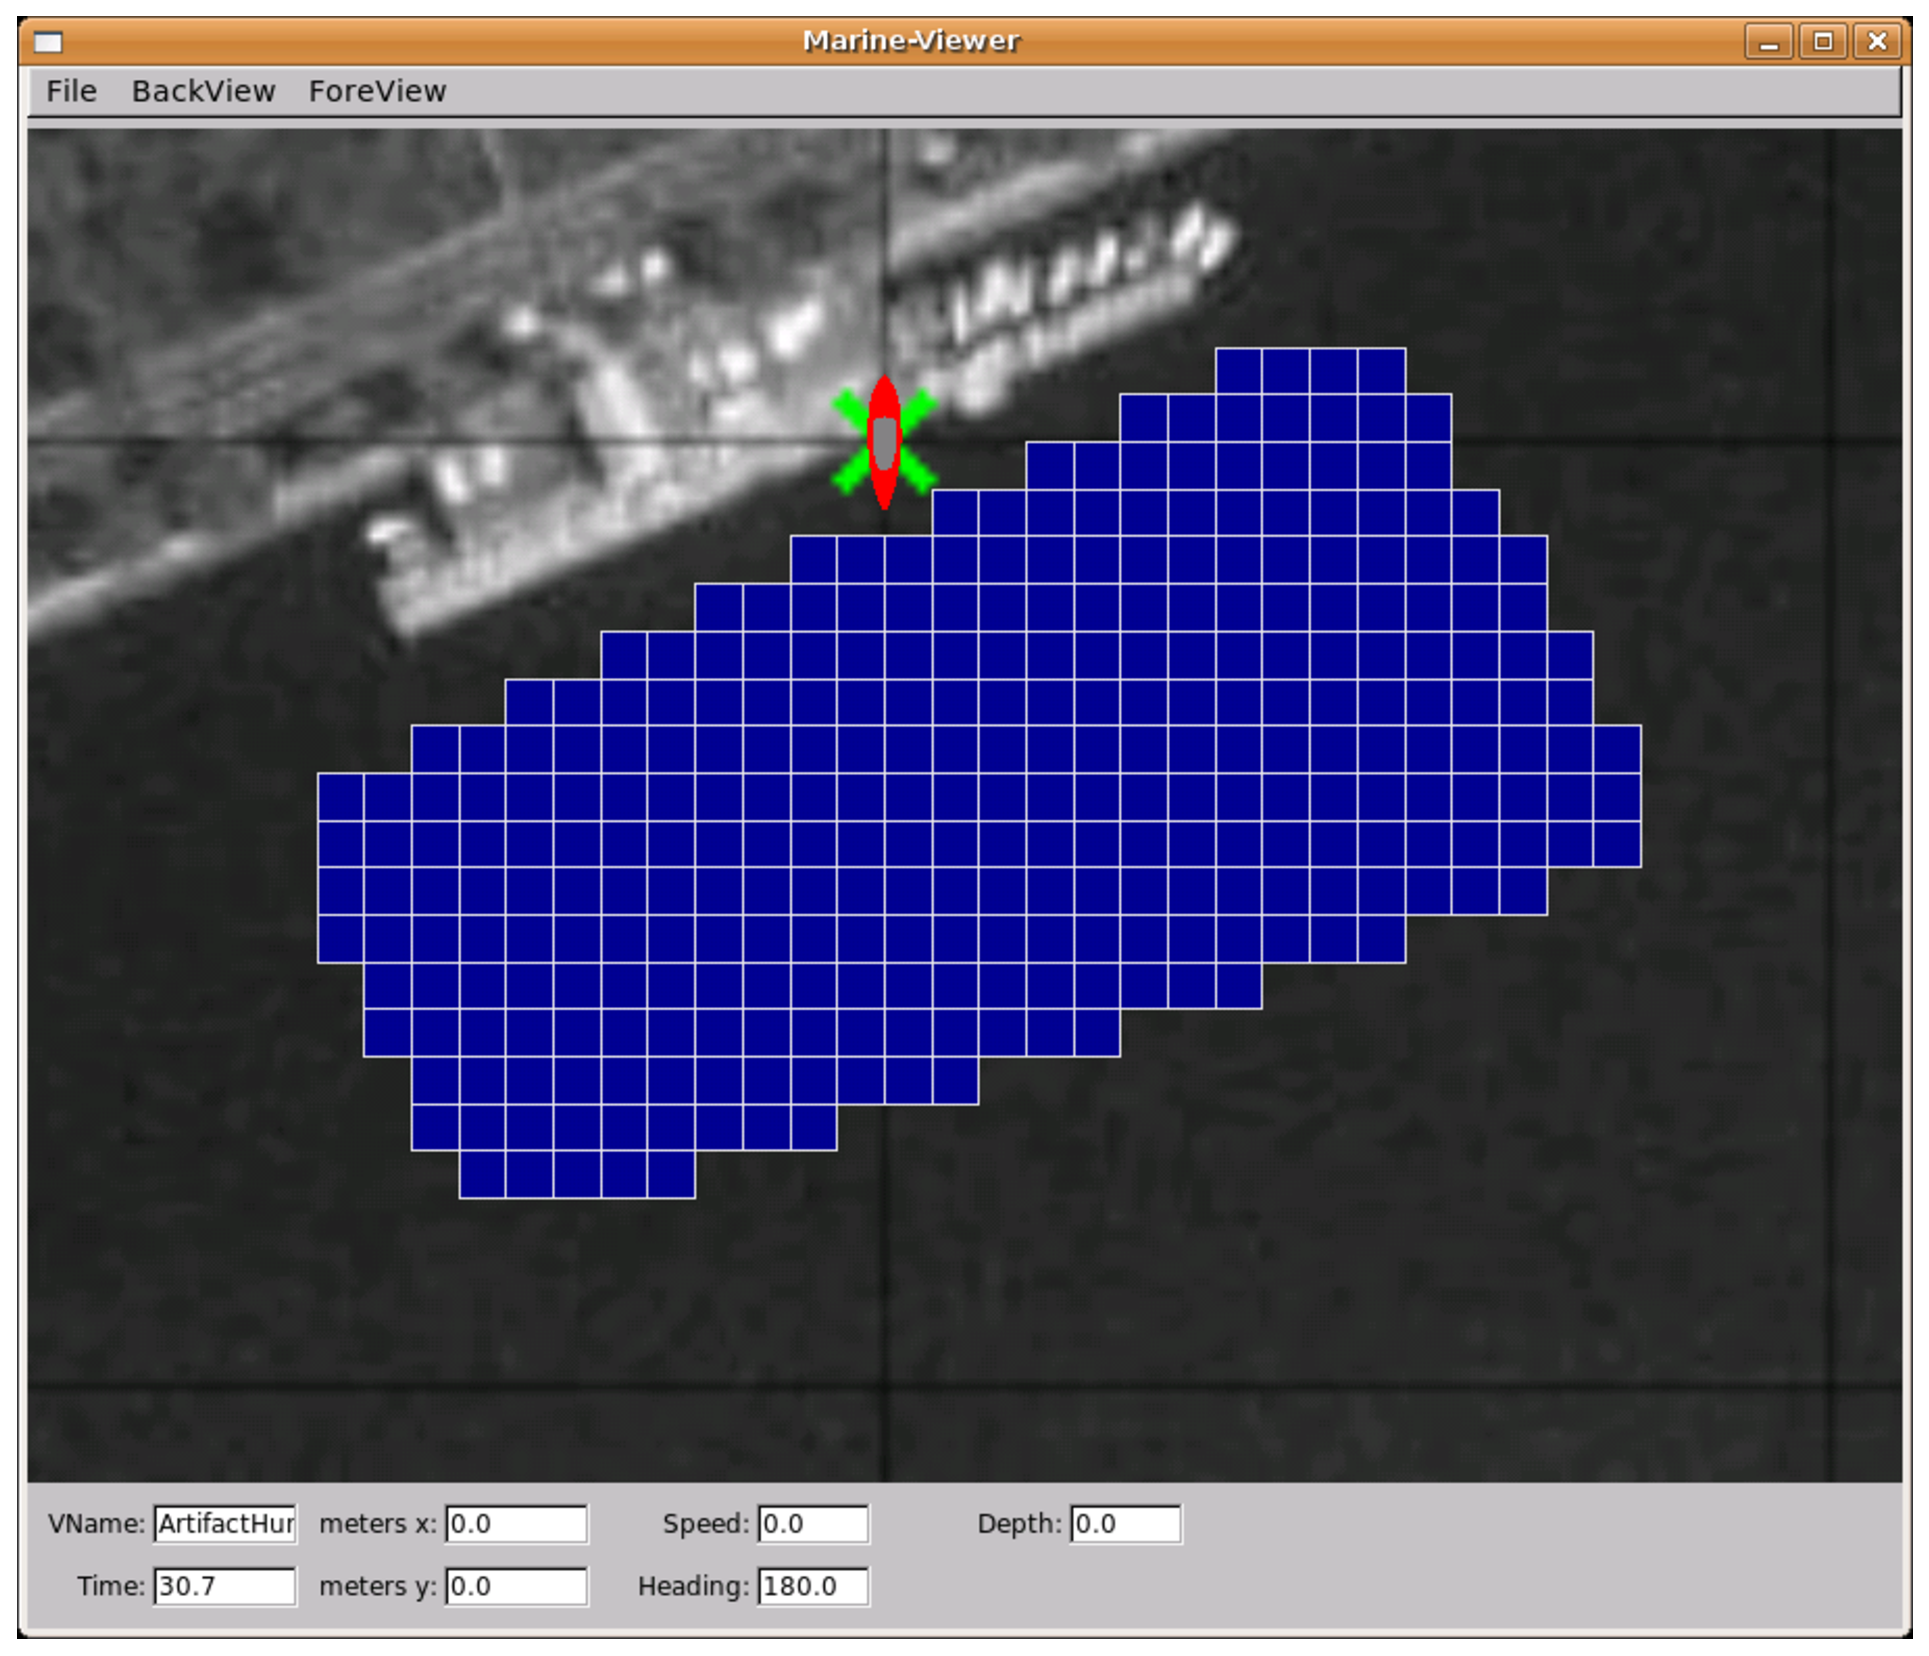
\includegraphics[width=2.5in]{figures/searchgrid}
\end{minipage}%
\caption{A search grid defined over a search area.} 
\end{figure}

There are two main MOOS processes and one IvPHelm behavior that implement the artifact search system.  pSensorSim simulates the output of an imaginary sensor in a simulated artifact field.  pArtifactMapper takes the output of pSensorSim, fuses it with output from other artifact search platforms in the area, and produces a likelihood map of artifacts in the search region.  The IvPHelm behavior, bhv\_SearchGrid, provides desired heading and speed information to the helm to optimize the user's utility function (e.g. mapping an entire field with 95\% confidence in the least amount of time).
% \begin{figure}[ht]
% \begin{minipage}[c]{0.5\textwidth}
%   \centering \includegraphics[width=2.5in]{figures/concept1.eps}
% \end{minipage}%
% \caption{The helm as a process in a MOOS community. \label{conceptone}} 
% \end{figure}


\section{pSensorSim}
\label{pSensorSim}

pSensorSim is composed of two C++ classes, ArtifactField and SensorModel.  Most users will not directly use these classes and will instead interact with them through the MOOSApp pSensorSim.

\subsection{Class ArtifactField}
\label{classArtifactField}
ArtifactField simulates an artifact field.  Internally, it is a vector of strings, where each string represents one artifact.  An artifact string consists of a comma separated list of equal-sign delimited variable-value pairs.  For example, ``Var1=val1,Var2=val2,Var3=val3''.  This structure makes it easy to add new traits to artifacts without having to change much code in other segments.

ArtifactField can return a list of artifacts within a 2D rectangle or circle when the artifact strings contain both ``X=xval'' and ``Y=yval'' (e.g ``X=10,Y=4.5,TYPE=magnetic'').

\subsubsection*{Public Member Functions}
\begin{itemize}
\item void {\bf add\-Artifact} (std::string)
\begin{list}\small\item\em Puts an artifact into the field. \item\end{list}
\item void {\bf add\-Artifact} (double, double)
\begin{list}\small\item\em Constructs the proper string from an {\em x\/}, {\em y\/} pair. \item\end{list}
\item std::string {\bf get\-Artifact} (int) const 
\begin{list}\small\item\em Returns the artifact at index {\em i\/}. \item\end{list}
\item int {\bf size} () const
\begin{list}\small\item\em Returns the number of artifacts in the field. \item\end{list}
\item std::vector$<$ std::string $>$ {\bf get\-Artifactbox} (double, double, double, double) const
\begin{list}\small\item\em Returns a vector of all artifacts within the 2D, X,Y box specified by the parameters. \item\end{list}
\item std::vector$<$ std::string $>$ {\bf get\-Artifactcircle} (double, double, double) const
\begin{list}\small\item\em Returns a vector of all artifacts within the 2D, X,Y circle specified by the parameters. \item\end{list}\end{itemize}

\subsection{Class SensorModel}
\label{classSensorModel}
SensorModel models the output of a specified sensor on a given ArtifactField.  After creating a SensorModel object, the programmer initializes the sensor by calling {\bf set\-Sensor\-Model} with the name of the model to simulate (currently, only a fixed radius, guaranteed-detection sensor is modeled, ``fixedradius'') and setting the detection radius using {\bf set\-Sensor\-Radius}.  The programmer can query the sensor by calling {\bf query\-Sensor} with a query string that is determined by the sensor.  For the fixed-radius sensor, the query string should contain the current X and Y values, e.g. ``X=4.5,Y=1.3''.

\subsubsection*{Public Member Functions}
\begin{itemize}
\item bool {\bf set\-Sensor\-Model} (std::string const)
\begin{list}\small\item\em Currently accepted value is ``fixedradius''. \item\end{list}
\item void {\bf set\-Sensor\-Radius} (double)
\begin{list}\small\item\em The sensor radius must be a non-negative value. \item\end{list}
\item double {\bf get\-Sensor\-Radius} () const
\item std::vector$<$ std::string $>$ {\bf query\-Sensor} (std::string const, {\bf Artifact\-Field} const \&) const
\begin{list}\small\item\em \begin{description}
\item[Parameters:]
\begin{description}
\item[{\em Art\-Field}]is a reference to an artifact field \end{description}
\end{description}
\item\end{list}\end{itemize}

\subsection*{Private Member Functions}
\begin{itemize}
\item std::vector$<$ std::string $>$ {\bf query\-FRSensor} (std::string const, {\bf Artifact\-Field} const \&) const
\begin{list}\small\item\em A private method for querying a fixed-radius sensor. \item\end{list}\end{itemize}
\subsection*{Private Attributes}
\begin{itemize}
\item double {\bf d\-Sensor\-Radius}
\begin{list}\small\item\em The maxiumum effective sensor radius. \item\end{list}
\item std::string {\bf s\-Sensor\-Type}
\begin{list}\small\item\em A string holding the current sensor type. \item\end{list}\end{itemize}

\subsection{MOOSApp pSensorSim}
\label{apppSensorSim}
Combining these two classes and creating a MOOSApp, we get Fig.~\ref{fig:sensorsim}.

\img[width=.5\linewidth]{figures/sensorsim}{A class diagram for pSensorSim}{fig:sensorsim}

\subsubsection{Configuration}
The pAntler configuration block for pSensorSim looks like this:
\scriptsize
\begin{verbatim}
//------------------------------------------
// pSensorSim config block
ProcessConfig = pSensorSim
{
   AppTick   = 4
   CommsTick = 4
   
   ArtifactFile = mines.art
   Artifact = X=10,Y=10
   Sensor = FixedRadius
   Sensor_Radius = 10   
}
\end{verbatim}
\normalsize

\begin{hangpar}{\pin}{\var{ArtifactFile: }}
Optional. This is the path to a file that contains lines of the form ``Artifact = artifactstring''.  Blank lines are ignored.  Useful for adding randomly generated fields using artfieldgenerator.  See Appendix~\ref{app:artfieldgenerator}
\end{hangpar}

\begin{hangpar}{\pin}{\var{Artifact: }}
Optional. An artifact string to add to the artifact field.
\end{hangpar}

\begin{hangpar}{\pin}{\var{Sensor: }}
Mandatory. A string containing the sensor type to simulate.  Only FixedRadius is currently implemented.
\end{hangpar}

\begin{hangpar}{\pin}{\var{Sensor\_Radius: }}
Optional. The effective radius of the FixedRadius sensor.  Defaults to 10m, must be non-negative.
\end{hangpar}

\subsubsection{MOOS Variables}
\paragraph{Subscribes}
\begin{hangpar}{\pin}{\var{NAV\_X} and \var{NAV\_Y: }}
Used to determine the current location of the sensor.  Uses only the most recently received value.
\end{hangpar}
\paragraph{Publishes}
\begin{hangpar}{\pin}{\var{DETECTED\_ARTIFACT: }}
A string that contains the output of the sensor evaluated at the current position.  For the fixed radius sensor, the output is ``X=x\_val,Y=y\_val,Prob=probability''.  pArtifactMapper subscribes to this variable.
\end{hangpar}

\begin{hangpar}{\pin}{\var{VIEW\_POLYGON: }}
On each iteration, plots a 12-point hexagon of radius 10-m around the kayak labelled with the community name.  An example string is ''radial:x,y,10,12,0.0,ArtifactHunter''.
\end{hangpar}

\begin{hangpar}{\pin}{\var{VIEW\_POINT: }}
Published once on startup for each artifact loaded into the artifact field.
\end{hangpar}


\section{pArtifactMapper}
\label{pArtifactMapper}

pArtifactMapper implements MOOSApp functionality for the XYArtifactGrid C++ class.

\subsection{XYArtifactGrid}
\label{XYArtifactGrid}

XYArtifactGrid is a simple class derived from XYGrid.  Using the functionality of XYGrid, this class is able to instantiate a search grid on top of a given search area.  Each cell in this search grid has a value member and a utility member.  The value member can be set to any double.  The utility member is bounded by the minimum and maximum utilities set by the programmer.

\subsection{pArtifactMapper}
The simple class diagram for pArtifactMapper is shown in Fig.~\ref{fig:artifactmapper}.

\img[width=\linewidth]{figures/artifactmapper}{A class diagram for pArtifactMapper}{fig:artifactmapper}

The pAntler configuration block for pArtifactMapper looks like this:
\begin{verbatim}
//------------------------------------------
// pArtifactMapper config block
ProcessConfig = pArtifactMapper
{
   AppTick   = 4
   CommsTick = 4
   
   GridPoly =  poly:label,A:-60,-40:50,10:80,-40:-40,-80
   GridSize = 5.0
   GridInit = .5
}
\end{verbatim}

\begin{itemize}
\item {\bf GridPoly}  A valid polygon initialization string (must be convex) that covers the search area.
\item {\bf GridSize}  The width/height of each cell in the search grid in meters.
\item {\bf GridInit}  The initializing value for each cell.
\end{itemize}


\section{bhv\_SearchGrid}
\label{bhvSearchGrid}


\section{Example Missions}
\label{examples}

\subsection{Tutorial}
\label{ex:tutorial}
This example gives a tutorial on how one might go about creating and executing a mission to search for artifacts.

\subsubsection{Setup}
\label{ex:tutorial:setup}
The first step is to define the search area.  Using polyview, click on a few points (maintaining a convex polygon) to create the search area and export the polygon string.

\img[width=\linewidth]{figures/01polyview}{Defining the search area in polyview}{fig:01polyview}

We now generate a random artifact field for searching.  In the directory you want to run your mission file from:

{\tt artfieldgenerator label,A:-119,-60:109,40:130,-97:-55,-156 .25 25 > mines.art}

This generates some random artifacts:

\begin{verbatim}
head -4 mines.art 
ARTIFACT = X=92.5,Y=26.25
ARTIFACT = X=59.25,Y=-47.25
ARTIFACT = X=-30.25,Y=-60.25
ARTIFACT = X=88.5,Y=-85.25
\end{verbatim}

The next setup task is to create the MOOS mission file.  See Appendix~\ref{app:tutorialmission} for a working example.  The relevant portions are printed below:
\begin{verbatim}
//------------------------------------------
// pSensorSim config block
ProcessConfig = pSensorSim
{
   AppTick   = 4
   CommsTick = 4
   
   ArtifactFile = mines.art
   Artifact = X=10,Y=10
   Sensor = FixedRadius
   Sensor_Radius = 10   
}

//------------------------------------------
// pArtifactMapper config block
ProcessConfig = pArtifactMapper
{
   AppTick   = 4
   CommsTick = 4
   
   GridPoly =  label,A:-119,-60:109,40:130,-97:-55,-156
   GridSize = 5.0
   GridInit = .5
}
\end{verbatim}

We also need to configure the helm to run a simple behavior to search over the search area.  To do this we first need to create a sequence of points for the vehicle to search over.  Load polyview with the previously defined search area (pass polyview a file with a line that reads ``Polygon = polystring'' to get it to load) and create a new ``polygon'' (not really a polygon as it will not be convex) whose points are the points in the lawn-mower pattern.  See Fig.~\ref{fig:02lawnmower} for an example.  Export this sequence of points and put it in the bhv file.  See Appendix~\ref{app:tutorialbehavior} for an example behavior.

\img[width=\linewidth]{figures/02lawnmower}{Defining the lawn-mower pattern in polyview}{fig:02lawnmower}

\subsubsection{Launch}
\label{ex:tutorial:launch}
After getting setup for the mission, we invoke it with {\tt pAntler~mission.moos}.  The display should look like Fig.~\ref{fig:04missionstart}.  The blue grid is the search grid, the light blue dots are artifacts, and the circle around the kayak is the detection radius.  To start the helm, in iRemote, set Deploy = TRUE (key 4), and then relinquish manual control ('o').

\img[width=\linewidth]{figures/03missionstart}{pMarineViewer at the beginning of an artifact search mission}{fig:04missionstart}

The kayak will now loop through the points defined in the lawn-mower pattern and the various displays will update accordingly.


\small
\bibliographystyle{plain} 
\bibliography{biblio}

\newpage
\appendix
\section{artfieldgenerator}
\label{app:artfieldgenerator}
artfieldgenerator is a command line tool for generating random artifact fields for testing various behaviors and algorithms.

To use artfieldgenerator:

\scriptsize
{\tt artfieldgenerator poly\_string step\_size num\_artifacts}
\normalsize

\begin{hangpar}{\pin}{\var{poly\_string: }}
A valid polygon initialization string (convex).  All of the artifacts will be contained within this polygon.  Some artifacts, however, may exist outside a search grid, depending on the size of the grid elements.
\end{hangpar}

\begin{hangpar}{\pin}{\var{step\_size: }}
Where to step the X, Y values (e.g. .25 generates values in .25 increments)
\end{hangpar}

\begin{hangpar}{\pin}{\var{num\_artifacts: }}
Number of unique artifacts to generate
\end{hangpar}

The output of artfield generator is written to standard out, so it is often redirected to a file for later use:

\scriptsize
{\tt artfieldgenerator label,A:-60,-40:50,10:80,-40:-40,-80 .25 25 > mines.art}
\normalsize

\section{Tutorial Mission}
\label{app:tutorialmission}
Line break in polygon string is provided for readability only.

File: mission.moos
\scriptsize
\verbatiminput{missions/mission.moos}
\normalsize

\section{Tutorial Behavior}
\label{app:tutorialbehavior}
Line breaks in point list are provided for readability only.

File: artifactsearch.bhv
\scriptsize
\verbatiminput{missions/artifactsearch.bhv}
\normalsize

%\input{sec_bravo_moos}
%\input{sec_charlie_moos}

\end{document}
